\begin{center}
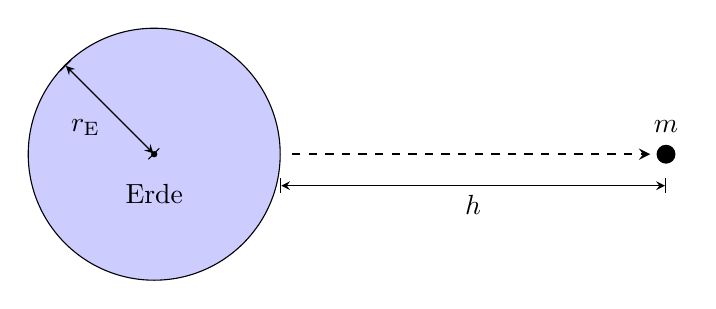
\begin{tikzpicture}[>=stealth]
 \fill[blue!20] (0,0) circle (1.6);
 \draw (0,0) circle (1.6);
 \fill (0,0) circle (0.04);
 \node at (0,-0.5) {Erde};

 \draw[|<->|] (0,0) -- (-1.131,1.131) node[midway, below left] {$r_\mathrm{E}$};
 \fill (6.5,0) circle (0.12);
 \node[above] at (6.5,0.15) {$m$};
 \draw[|<->|] (1.6,-0.4) -- (6.5,-0.4) node[midway, below] {$h$};
 \draw[->, thick, dashed] (1.75,0) -- (6.3,0);
\end{tikzpicture}
\end{center}

Bei dieser Höhe ändert sich die Gravitationskraft stark, die Formel $m\,g\,h$ gilt nicht. Die Gravitationsenergie ist $E_\mathrm{p} = -G\,\frac{M_\mathrm{E}\,m}{r}$ (Nullpunkt im Unendlichen). Die erforderliche Energie ist ihre Zunahme zwischen $r_\mathrm{E}$ und $r_\mathrm{E}+h$:
\begin{align}
 \Delta E &= -G\,\frac{M_\mathrm{E}\,m}{r_\mathrm{E}+h}-\left(-G\,\frac{M_\mathrm{E}\,m}{r_\mathrm{E}}\right) = \EHF \\
   &= \ncG\cdot\MEr\cdot\mSa\cdot\left(\frac{1}{\REr}-\frac{1}{\REr+\hSa}\right) \\
   &= \EH \approx \result{\EHP{9}{2}}
\end{align}
mit $M_\mathrm{E} = \MErO$ und $r_\mathrm{E} = \RErO$ (FoTaBe S.~209). Soll der Satellit in dieser Höhe die Erde umkreisen, braucht er zusätzlich kinetische Energie.
